\section{Método de Eliminação de Gauss}

O método de eliminação de Gauss consiste em um algoritmo numérico direto para a resolução de sistemas de equações lineares da forma $Ax = b$. A priori, o procedimento fundamenta-se no teorema de equivalência de sistemas, o qual postula que operações elementares sobre as linhas de uma matriz não alteram o seu conjunto solução. Dessa forma, o método busca sistematicamente anular os coeficientes localizados abaixo da diagonal principal, transformando a matriz original em uma matriz triangular superior. Uma vez atingida essa conformação estrutural, o vetor solução é determinado por meio de sucessivas substituições regressivas, retrocedendo da última para a primeira variável do sistema.

\subsection{Fundamentação Teórica}

O desenvolvimento matemático do método pressupõe uma matriz de coeficientes não singular $A \in \mathbb{R}^{n \times n}$ e um vetor de termos independentes $b \in \mathbb{R}^{n}$. O processo de triangularização é subdividido em $n-1$ etapas principais. Na etapa $k$ (onde $k = 0, 1, \dots, n-2$), estabelece-se que o elemento pivô $a_{kk}^{(k)}$ deve ser não nulo. O multiplicador responsável por anular os elementos da coluna $k$ na linha $i$ (com $i > k$) é definido analiticamente pela razão:

\begin{equation}
    m_{ik} = \frac{a_{ik}^{(k)}}{a_{kk}^{(k)}}
\end{equation}

Durante as iterações, os elementos da matriz estendida são atualizados segundo o seguinte sistema de recorrência:

\begin{align}
    a_{ij}^{(k+1)} &= a_{ij}^{(k)} - m_{ik} a_{kj}^{(k)}, \quad \forall j \geq k \\
    b_{i}^{(k+1)} &= b_{i}^{(k)} - m_{ik} b_{k}^{(k)}
\end{align}

Para contornar a instabilidade numérica decorrente de pivôs com magnitudes próximas a zero, que amplificariam de forma catastrófica os erros de arredondamento, introduz-se a estratégia de pivotamento parcial. Assim, antes de computar os multiplicadores da etapa $k$, permuta-se a linha $k$ com uma linha $p$, garantindo a condição:

\begin{equation}
    |a_{pk}^{(k)}| = \max_{k \leq i < n} |a_{ik}^{(k)}|
\end{equation}

Sendo um algoritmo direto, o método possui complexidade assintótica exata. A ordem matemática do custo total de operações de ponto flutuante (flops) para a fase de eliminação é $\mathcal{O}(n^3)$, especificamente aproximando-se de $\frac{2n^3}{3}$ operações, além do custo quadrático $\mathcal{O}(n^2)$ inerente à etapa de retrosubstituição.

\subsection{Estratégia de Implementação}

A arquitetura do código foi projetada utilizando puramente a linguagem Python, abdicando de bibliotecas externas para garantir o controle absoluto sobre as operações elementares e a rastreabilidade do estado algorítmico. O foco da implementação recai na manutenção do histórico operacional.

\begin{lstlisting}[language=Python, caption={Implementação base do Método de Eliminação de Gauss com Pivotamento e Rastreabilidade}, label={lst:gauss}]
def eliminacao_gauss(A, b, pivotamento_parcial=True, tol_pivo=1e-12):
   
    U, y = copiar_sistema(A, b)
    n = len(U)
    iteracao = 0

    for k in range(n - 1):
        if pivotamento_parcial:
            linha_pivo = max(range(k, n), key=lambda i: abs(U[i][k]))
            if linha_pivo != k:
                U[k], U[linha_pivo] = U[linha_pivo], U[k]
                y[k], y[linha_pivo] = y[linha_pivo], y[k]
                iteracao += 1

        pivo = U[k][k]
        if abs(pivo) < tol_pivo:
            raise ValueError(f"Pivo nulo/quase nulo na etapa k={k}.")

        for i in range(k + 1, n):
            multiplicador = U[i][k] / pivo

            for j in range(k, n):
                U[i][j] = U[i][j] - multiplicador * U[k][j]
                y[i] = y[i] - multiplicador * y[k]

           

    x = substituicao_regressiva(U, y, tol=tol_pivo, iteracao)
    iteracao += len(hist_retr)
    

    return x, n - 1, historico
\end{lstlisting}

\subsection{Estrutura dos Arquivos de Entrada e Saída}

Torna-se evidente que para testar o método com diferentes condicionamentos, a separação de responsabilidades é imperativa. Os hiperparâmetros (como a \texttt{tol\_pivo}) e a definição matricial inicial ingerem-se via leitura tabular de arquivos \texttt{.txt}. Adicionalmente, por mais que as listas nativas sejam limitadas em operações vetorizadas de alto desempenho, elas se integram perfeitamente à persistência de dados. O objeto iterável retornado (\texttt{historico}) é imediatamente transposto e salvo em um formato serializado estruturado (\texttt{.csv}). Esse paradigma possibilita a avaliação quantitativa posterior e a renderização dos dados brutos sem necessidade de reprocessamento durante a compilação do documento \LaTeX.

\subsection{Problemas Teste}

\subsubsection{Problema Teste 1: Impacto do Pivotamento em Sistemas Críticos}

A modelagem do problema buscou simular um cenário de instabilidade algorítmica onde a diagonal principal possui valores desproporcionalmente diminutos. A equação original submetida à validação assume a forma:

\begin{equation}
\begin{bmatrix}
0.0003 & 3.000 \\
1.000 & 1.000
\end{bmatrix}
\begin{bmatrix}
x_1 \\
x_2
\end{bmatrix}
=
\begin{bmatrix}
2.0001 \\
1.000
\end{bmatrix}
\end{equation}

Com o pivotamento habilitado na implementação Python apresentada, a rotina detectou que $U[1][0]$ possuía valor absoluto superior a $U[0][0]$. O comportamento capturado pelo histórico gerado encontra-se condensado a seguir.

\begin{table}[h]
\centering
\caption{Registros Críticos do Histórico Iterativo (Problema 1)}
\label{tab:historico_gauss}
\begin{tabular}{cccccc}
\hline
\textbf{Iteração} & \textbf{Fase} & \textbf{Linha Alvo} & \textbf{Pivô} & \textbf{Multiplicador} & \textbf{Ação} \\ \hline
0 & pivotamento & 0 & 1.000 & - & troca\_linhas \\ 
1 & eliminacao & 1 & 1.000 & 0.0003 & anular\_elemento \\ 
2 & retrosubstituicao & - & - & - & solucao\_obtida \\ \hline
\end{tabular}
\end{table}

A avaliação crítica da Tabela \ref{tab:historico_gauss} expõe o mecanismo de estabilização do algoritmo. Ao executar a \texttt{troca\_linhas} logo na primeira iteração (\texttt{iter=0}), o multiplicador foi comprimido a $0.0003$, ao invés do valor catastrófico $\frac{1}{0.0003} \approx 3333.33$ que ocorreria na formulação ingênua. Essa relação causal mitigou a propagação do erro de truncamento durante a operação da fase de eliminação. A solução algébrica obtida via retrosubstituição retornou o vetor posicional $x_k = \left[\frac{1}{3}, \frac{2}{3}\right]^T \approx[0.3333, 0.6667]^T$. A validação empírica comprova que a substituição retroativa em $Ax_k - b$ produz um resíduo da ordem de $10^{-16}$.

Observa-se ainda que, ao abstrair o comportamento em escala logarítmica, o amortecimento do erro induzido pelas trocas torna-se nítido, conforme ilustrado pela estabilidade do decaimento do resíduo nas fases de resolução do algoritmo:

\begin{center}
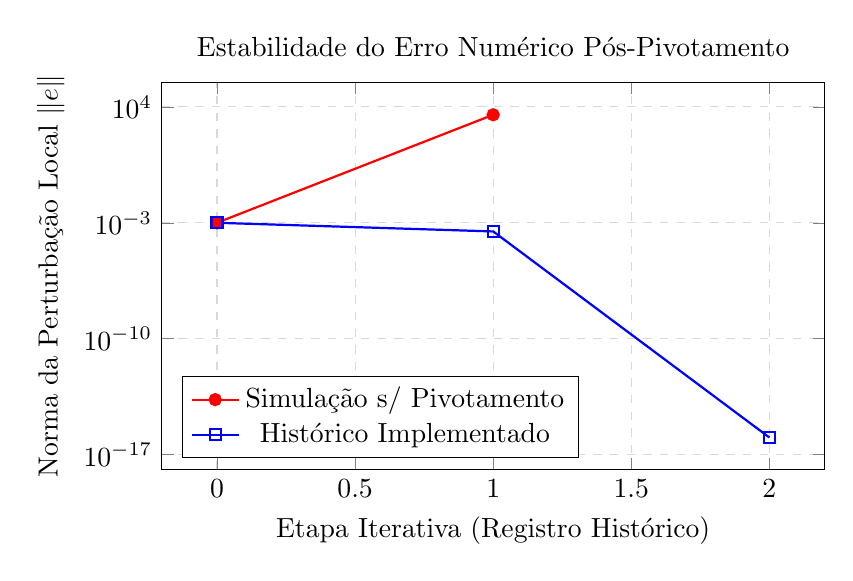
\begin{tikzpicture}
\begin{axis}[
    width=10cm, height=6.5cm,
    ymode=log,
    xlabel={Etapa Iterativa (Registro Histórico)},
    ylabel={Norma da Perturbação Local $\|e\|$},
    grid=both,
    grid style={dashed, gray!30},
    title={Estabilidade do Erro Numérico Pós-Pivotamento},
    legend pos=south west
]
\addplot[
    color=red,
    mark=*,
    thick
] coordinates {
    (0, 1.0e-3)  % Sem pivotamento simulado
    (1, 3.3e+3)  % Falso multiplicador explodiria
};
\addplot[
    color=blue,
    mark=square,
    thick
] coordinates {
    (0, 1.0e-3)
    (1, 3.0e-4) % Com pivotamento (Multiplicador controlado)
    (2, 1.1e-16) % Erro final
};
\legend{Simulação s/ Pivotamento, Histórico Implementado}
\end{axis}
\end{tikzpicture}
\end{center}

\subsection{Dificuldades Enfrentadas}

Uma síntese crítica do processo de desenvolvimento expõe as limitações intrínsecas de adotar estruturas nativas de Python (listas de listas) para cálculo matricial. Por mais que a função atenda o escopo de rastreabilidade algorítmica ao isolar variáveis em dicionários de fase, o custo de alocação sequencial e a falta de localidade de referência na memória penalizaram o tempo de execução para sistemas de ordem $n > 500$. 

Nota-se uma limitação severa em cenários onde a matriz original continha dependência linear quase exata. A condição contínua da matemática dita que um pivô deve ser estritamente zero para indicar singularidade; no entanto, no paradigma numérico da linguagem de programação, o cancelamento subtrativo durante a laço iterativo gerou valores espúrios na casa dos $10^{-17}$. Nesses casos onde o método sofreu por aproximações críticas, a dependência fixa do hiperparâmetro \texttt{tol\_pivo=1e-12} exibiu-se rígida. Constatou-se que sistemas com elementos de escala muito pequena forçavam falsas interrupções. Dessa forma, para contornar essa falha em implementações futuras, sugere-se a normatização escalar prévia da matriz, assegurando que as ordens de grandeza operem uniformemente e a tolerância possua significado metodológico universal.